\documentclass{sig-alternate-05-2015}

\begin{document}

% Copyright
\setcopyright{acmcopyright}
%\setcopyright{acmlicensed}
%\setcopyright{rightsretained}
%\setcopyright{usgov}
%\setcopyright{usgovmixed}
%\setcopyright{cagov}
%\setcopyright{cagovmixed}


% DOI
\doi{TBD}

% ISBN
\isbn{TBD}

%Conference
\conferenceinfo{SAICSIT '16}{September 26--28, 2016, Johannesburg, South Africa}

%\acmPrice{\$15.00}

%
% --- Author Metadata here ---
\conferenceinfo{Solms, Coetzee}{'16 Johannesburg, South Africa}
%\CopyrightYear{2007} % Allows default copyright year (20XX) to be over-ridden - IF NEED BE.
%\crdata{0-12345-67-8/90/01}  % Allows default copyright data (0-89791-88-6/97/05) to be over-ridden - IF NEED BE.
% --- End of Author Metadata ---

\title{A case study of Agile practices applied to a project seeking DO-178 certification}

\numberofauthors{2} %  in this sample file, there are a *total*
\author{
\alignauthor
Dr Fritz Solms\\
%      \titlenote{Advisor}\\
	   \affaddr{Department of Computer Science}\\
       \affaddr{Faculty of Engineering, Built Environment}\\
       \affaddr{and Information Technology}\\
       \affaddr{University of Pretoria}\\
       \email{fsolms@cs.up.ac.za}  
\alignauthor
Kobus Coetzee\\
%	   \titlenote{Researcher}\\
       \affaddr{Graduate School of Technology Management}\\
       \affaddr{Faculty of Engineering, Built Environment}\\
       \affaddr{and Information Technology}\\
       \affaddr{University of Pretoria}\\
       \email{kobus@embeddedfool.net}
}

\maketitle
\begin{abstract}
This study measures the feasibility of applying agile software development practices to high reliability software projects seeking DO-178 certification. This is done by comparing two student developer teams completing two projects according to the same specifications. One team uses traditional waterfall development methodologies while the other uses agile methodologies. The teams are compared on the Robustness, Functionality delivered, Solution complexity, Certification effort required, Lines of code, Word count and Quality of the documentation delivered (TODO Review).
\end{abstract}


%
% The code below should be generated by the tool at
% http://dl.acm.org/ccs.cfm
% Please copy and paste the code instead of the example below. 
%
\begin{CCSXML}
<ccs2012>
 <concept>
  <concept_id>10010520.10010553.10010562</concept_id>
  <concept_desc>Computer systems organization~Embedded systems</concept_desc>
  <concept_significance>500</concept_significance>
 </concept>
 <concept>
  <concept_id>10010520.10010575.10010755</concept_id>
  <concept_desc>Computer systems organization~Redundancy</concept_desc>
  <concept_significance>300</concept_significance>
 </concept>
 <concept>
  <concept_id>10010520.10010553.10010554</concept_id>
  <concept_desc>Computer systems organization~Robotics</concept_desc>
  <concept_significance>100</concept_significance>
 </concept>
 <concept>
  <concept_id>10003033.10003083.10003095</concept_id>
  <concept_desc>Networks~Network reliability</concept_desc>
  <concept_significance>100</concept_significance>
 </concept>
</ccs2012>  
\end{CCSXML}

\ccsdesc[500]{Computer systems organization~Embedded systems}
\ccsdesc[300]{Computer systems organization~Redundancy}
\ccsdesc{Computer systems organization~Robotics}
\ccsdesc[100]{Networks~Network reliability}


%
% End generated code
%

%
%  Use this command to print the description
%
\printccsdesc

% We no longer use \terms command
%\terms{Theory}

\keywords{Project management, Agile, Waterfall, DO-178}

\section{Introduction}
Software development practices have progressed through a great many iterations since the first conference on software engineering sponsored and facilitated by NATO in 1968 \cite{Bauer_1968}. Since the 1970's the development of software for military use has been standardised by the US Department of Defence, eventually leading to the generation of thousands of military standards of the form MIL-STD's \cite{McDonald_2010}. These MIL-STD's for software developed eventually led to the creation of derivative standards for software development. 
\break
\break
But since software engineering spans such a wide field, several best practices have developed for each field, with standards bodies regulating proper implementation of the practices, for example the RTCA (Radio Technical Commission for Aeronautics) specified standards being used in the aeronautical industry, MISRA (Motor Industry Software Reliability Association) specified standards being used in the automotive industry and the ISO (International Standards Organisation) regulating medical device software.  Both these standards body has as its objective to guide their industries to ensure the development of products that are safe, reliable, robust and adheres to minimum operational performance requirements.
\break
\break
The RTCA has published the DO-178C \cite{RTCA_2012} specification for "Software Considerations in Airborne Systems and Equipment Certification". MISRA has published the MISRA-C:2012 \cite{MISRA_2012} specification for "Guidelines for the use of the C language in critical systems". ISO has published the IEC 62304 \cite{Jordan_2006} specification for "Medical Device Software - Software Lifecycle Processes".
\break
\break
These standards prescribe a strict adherence to process and fixed design and implementation life cycles, but software development best practises experienced a paradigm shift the last decade with the coming of agile methodologies. Software development methodologies such as Scrum and Kanban can in some ways be considered the agile equivalents to the RTCA and MISRA standards. Furthermore agile methodologies have been shown to mostly result in improved software delivery times, software quality and client satisfaction with the end product \cite{Armbrust_2011}.
\break
\break
Even so, agile development is only practiced in a certain subset of software industries, mainly consumer software development \cite{Diebold_2014}. Two software industries that have remained largely immune to agile development practices and still mainly done with 1970's era waterfall methodologies is military and safety critical software. Contrast for instance RTCA's and MISRA's focus on safety, reliability, robustness and minimum operational performance mainly through rigid process and verification, with the agile manifesto \cite{Beck_2001}:
\break
\break
\textit{
	"We are uncovering better ways of developing software by doing it and helping others do it. Through this work we have come to value:
	\begin{itemize}
		\item Individuals and interactions over Processes and tools
		\item Working software over Comprehensive documentation
		\item Customer collaboration over Contract negotiation
		\item Responding to change over Following a plan
	\end{itemize}
	That is, while there is value in the items on the right, we value the items on the left more."
}

\section{Literature survey}
Very little research has been generated on the application of agile methods to highly regulated industries. Diebold \cite{Diebold_2014} did systematic study on agile penetration in various industries.

\begin{figure}[t!]
	\centering
	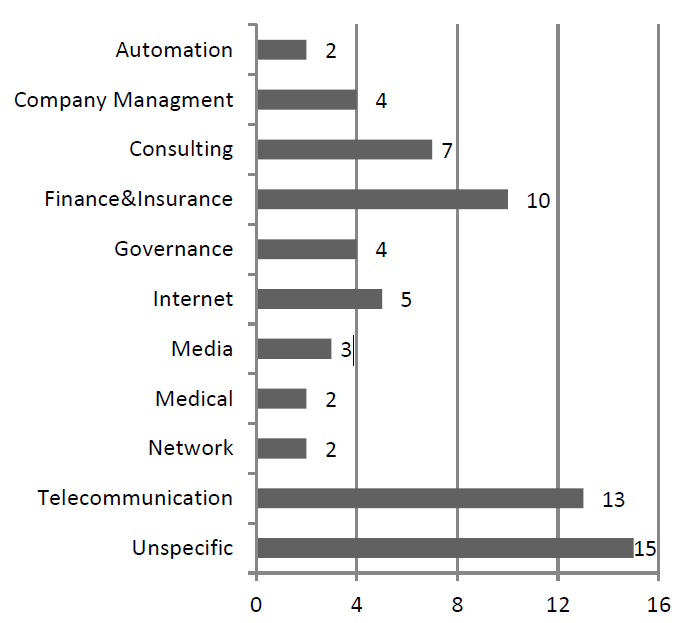
\includegraphics[width=90mm]{DieBold2014.png}
	\caption{Agile distribution across domains \cite{Diebold_2014} \label{overflow}}
\end{figure}

Note the low occurrence of agile in the automation and medical industries. But problematic also is getting to a clear definition of what exactly agile software development entails. If the difference can only be regarded as iterative vs. incremental development practices, then agile methods have been in development since the 1970's \cite{Larman_2003}. The latest iteration and most popular form of agile methods takes the shape of SCRUM, a process which specifies short development sprints of roughly two weeks in which certain developmental goals are specified and the team attempts to satisfy these goals. Cardazo \cite{Cardozo_2010} did a literature review and found SCRUM did to lead to productivity improvements, but did not investigate if organisational make-up or the industry the company operates in have any effect. Also these findings are still very recent, and more in depth analysis is required.   

A couple of case studies have been performed on implementing agile methodologies in regulated industries. Fitzgerald \cite{Fitzgerald_2013} found tension points when implementing a SCRUM process in a case study where the company and product had to comply with several FDA, ISO, IEC and ISPE regulations. These tension points were in quality assurance, safety and security, effectiveness, traceability, verification and validation. But even so it was found that agile can be suitable and even bring about improvements to regulated industry if tailored correctly. 

Shenvi \cite{Shenvi_2014} also investigated if improvements can be made in the development of medical equipment when employing techniques from six sigma and agile, while complying with regulatory standards. A theoretical model was developed, and employed as a case study, resulting in improvements in productivity and a decrease in defects in the final product in the period the model was used between 2010 and 2013. It is unknown if wider applicability of the model exists for other industries with other certification requirements. 

Hrgarek \cite{Hrgarek_2012} pointed to further difficulties companies face in the medical device manufacturing industry when trying to employ agile methods while staying compliant with regulations. It is unclear if the case study was successful in employing agile methods into the development process.

Glas \cite{Glas_2009} investigated a case in the application of agile methods in a aviation manufacturing setting, and identified open tool platforms and open design to be beneficial. The paper also mentioned regulatory difficulties as a problem for agile adoption, although this was not the focus of the study. 

In addition to agile methodologies such as SCRUM and Kanban etc, improvements have been made in developmental tools that aid in agile development. These tools include agile centric project management software, CI (Continuous integration), CD (Continuous deployment), Unit testing, TDD (Test driven development), BDD (Behaviour driven development), pair programming and others. 

Sfetsos \cite{Sfetsos_2010} did a literature survey and investigated which of the different agile tools does indeed provide improvements in product quality, and found TDD and pair programming to be beneficial. It should be noted that the study was performed in 2010, and a lot of improvements to agile has happened since then.

Causevic \cite{Causevic_2011} investigated uptake of TDD in industrial settings, and found the following limiting factors: increased development time, insufficient TDD experience/knowledge, lack of upfront design, domain and tool specific issues, lack of developer skill in writing test cases, insufficient adherence to TDD protocol, and legacy code. It is uncertain what is meant with an industrial setting, and if the companies involved was already engaged in other agile practices. 
 
Boehm \cite{Boehm_2003} shows that a balance between planned and agile methodologies can be found and formulates a strategy to arrive at such a balance. This paper is quite dated, especially given the velocity that agile is developing at, but represents a seminal work in blending agile and planned approaches from which several derivative works were produced. 

But even with the relatively slow uptake of agile in DO-178 projects, some work has been done on what high reliability agile would look like. The FDA (US Food and Drug Administration) released TIR45 \cite{AAMI_TIR45_2012}, which prescribes the application of agile software development practices for the development of safety critical medical devices seeking IEC 62304 certification. 

Furthermore Open-DO \cite{OPEN-DO_2010} is an initiative for the discussion of the application of agile methodologies to the DO-178C specification. Open-DO is facilitated a conference in 2010 in France for this purpose amongst others.     

\section{Survey on agile uptake in DO-178 projects}
For the purposes of this study survey responses were collected to answer the following questions about the current state of the DO-178 certified software industry:
\begin{enumerate}
	\item Is there a case for agile development within the DO-178 %environment?
	\item Is agile methods already being used within DO-178?
	\item To get a benchmark to measure if agile methods improve DO-178 %development? 
\end{enumerate} 

The survey was advertised on various DO-178 special interest groups and mailing lists, technical news aggregator sites as well emails sent to the authors personal contacts active with DO-178 development (This explains the high amount of South African respondents).

The survey was completed by 88 respondents, in various roles, with various team sizes and in various countries:
\begin{table}[t!]
	\centering
	\caption{Roles}
	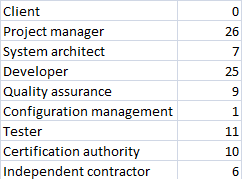
\includegraphics[width=60mm]{Roles.png}
\end{table}

\begin{figure}[t!]
	\centering
	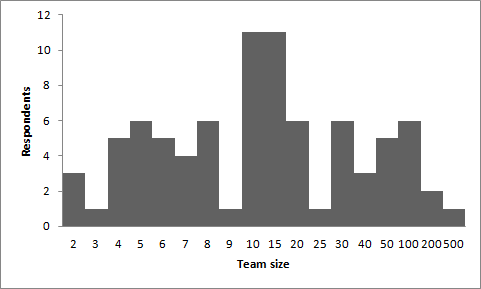
\includegraphics[width=90mm]{Teams.png}
	\caption{Team size}
\end{figure}

\begin{table}[t!]
	\centering
	\caption{Countries}
	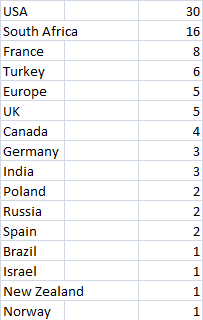
\includegraphics[width=50mm]{Countries.png}
\end{table}

Most respondents indicated they are still following the DO-178B specification and haven't switched over to the newer DO-178C specification which was released in January 2012.

\begin{table}[t!]
	\centering
	\caption{DO-178B and DO-178C use}
	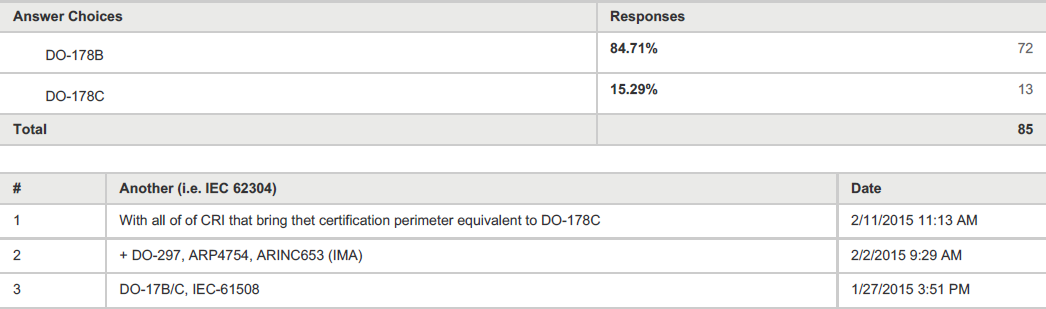
\includegraphics[width=90mm]{BvsC.png}
\end{table}

\subsection{A case for agile}
To determine if there is a case for the use of agile within DO-178, we looked at the current performance of DO-178 projects. This was done by asking the survey participants the following questions:

\begin{itemize}
	\item What was your last projects budget performance?
	\item What was your last project's delivery date performance?
	\item How many features was delivered according to the original specification?
	\item Was there any requests for additional features during the development? (Scope creep)
	\item Was there any requests for additional features after certification was complete? (Scope creep)
	\item In your opinion, does DO-178 increase the costs to a project? By how much?
\end{itemize}

These questions all measure the traditional improvements that agile can bring to a project, and as such any difficulty with these metrics should show that there is a case for the implementation of agile methodologies. The question is off course, at what cost.

\begin{table}[t!]
	\centering
	\caption{What was your last project's budget performance?}
	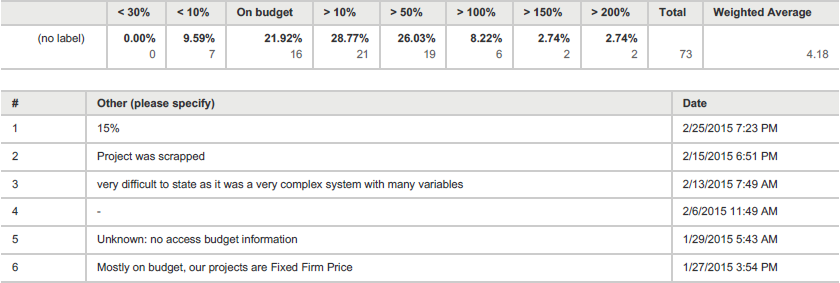
\includegraphics[width=90mm]{What_was_your_last_projects_budget_performance.png}
\end{table}

\begin{table}[t!]
	\centering
	\caption{What was your last project's delivery date performance?}
	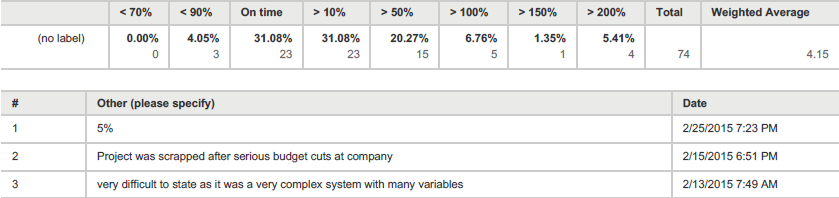
\includegraphics[width=90mm]{What_was_your_last_projects_delivery_date_performance.png}
\end{table}

\begin{table}[t!]
	\centering
	\caption{How many features was delivered according to the original specification?}
	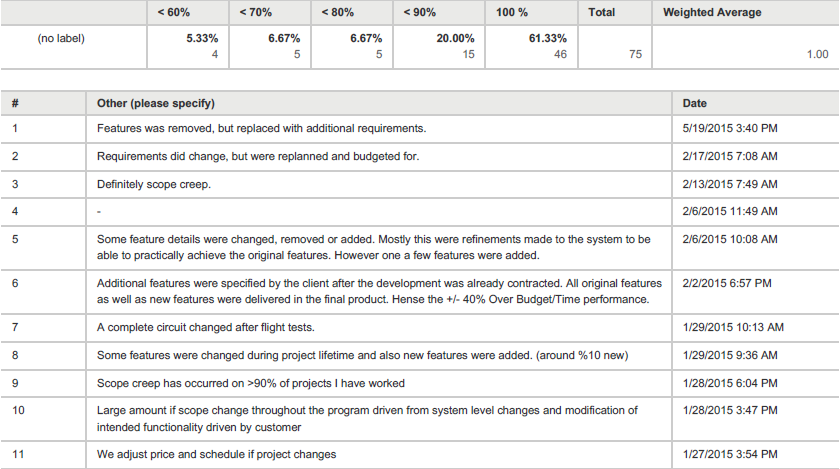
\includegraphics[width=90mm]{How_many_features_was_delivered_according_to_the_original_specification.png}
\end{table}

\begin{table}[t!]
	\centering
	\caption{Was there any requests for additional features during the development?}
	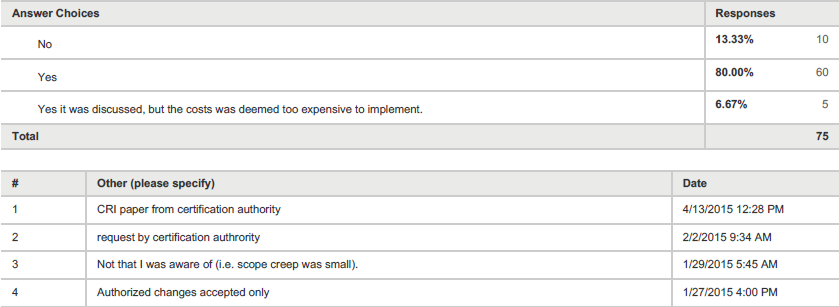
\includegraphics[width=90mm]{Was_there_any_requests_for_additional_features_during_the_development.png}
\end{table}

\begin{table}[t!]
	\centering
	\caption{Was there any requests for additional features after certification was complete?}
	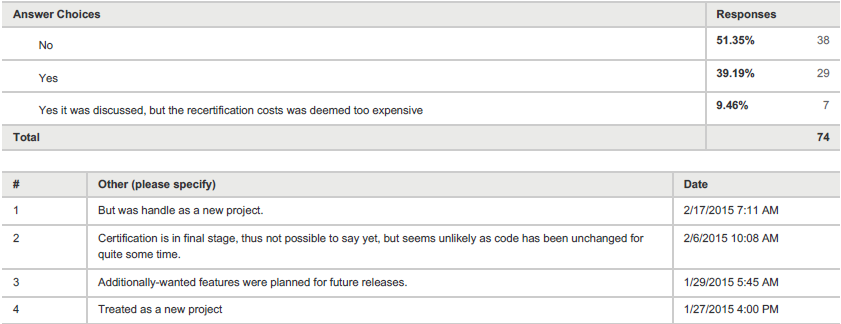
\includegraphics[width=90mm]{Was_there_any_requests_for_additional_features_after_certification_was_complete.png}
\end{table}

\begin{table}[t!]
	\centering
	\caption{In your opinion, does DO-178 increase the costs to a project?}
	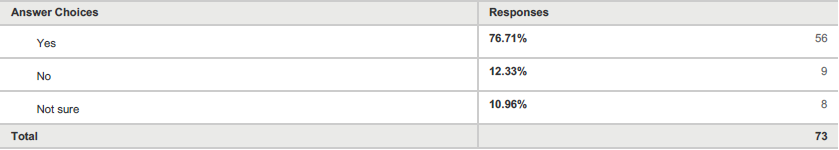
\includegraphics[width=90mm]{Does_increase_costs.png}
\end{table}

\begin{figure}[t!]
	\centering 
	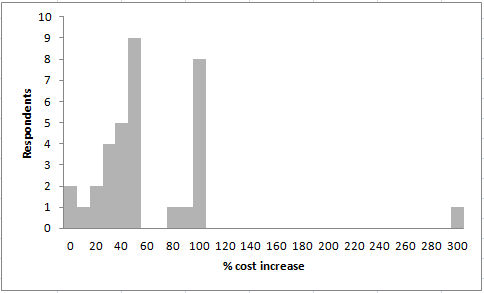
\includegraphics[width=90mm]{Cost_histogram.png}
	\caption{By how much does costs increase?}
\end{figure}
%\FloatBarrier

\subsection{Is agile being used}
We also wanted to find out to which extent agile techniques were already being practiced in the industry. But not everybody in the industry agrees as to the same definition of what an agile development approach is. As such we asked the respondents if they were using a waterfall, rational unified process, kanban and scrum approach. We correlated this metric by asking respondents to confirm if they were using various developmental tools, some being agile orientated and some waterfall orientated. These responses were then correlated with the developmental approach responses, and measured for correlation. 

We also asked the respondents if they felt the development approach was helpful or not in their completion of their projects:

\begin{table}[t!]
	\centering
	\caption{Waterfall vs agile use}
	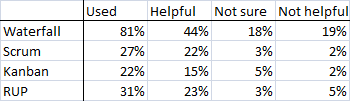
\includegraphics[width=60mm]{Agile_waterfall_uptake.png}
\end{table}

Note the percentages do not necessarily add up, as respondents may have filled in for multiple projects or multiple approaches may have been used within the same project (subcomponents for instance).    

\subsection{DO-178 benchmarks}
To measure the case study performance, the following benchmarks were gathered from the survey:

\begin{itemize}
	\item What is your \$ cost per line of code?
	\item What is your bugs per 1000 lines of code?
\end{itemize}

Off course these benchmarks presents difficulties of their own, such as inconsistent measuring, but the hope was that the benchmarks could be used as a measure to compare with the case study discussed later. Unfortunately this proved not to be that helpful.

\section{Conceptual model}

The following conceptual model were developed, taking inputs from TIR45 \cite{AAMI_TIR45_2012} and Open-DO \cite{OPEN-DO_2010}, but also taking general agile development principles, especially SCRUM and applying it to the required DO-178 outputs and objectives.

\begin{figure}[t!]
	\centering 
	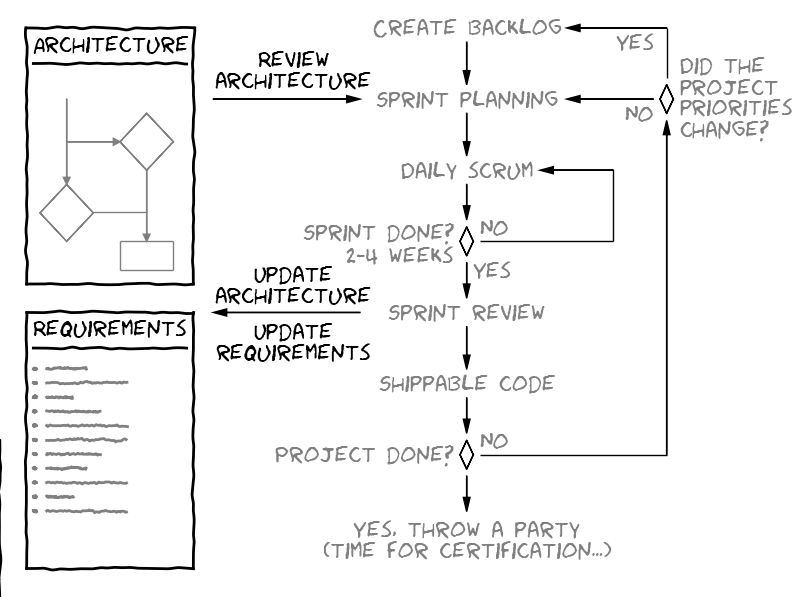
\includegraphics[width=90mm]{DO178_scrum.png}
	\caption{Agile DO-178 framework}
\end{figure}

The conceptual model is focused on bringing continuous integration and continuous deployment to a DO-178 environment. The purposes is to reduce costs through automation of repeated processes. Since DO-178B is a software quality assurance standard, not a software development standard, it does not impose any restrictions or considerations on how software is to be developed. It does however require the following list of deliverables, with the requirements for each depending on the criticality level chosen:
\\
\\
\textbf{Organisational deliverables}
(These can be re-used across multiple projects, if the projects are similar enough off course):

\begin{itemize}
	\item Software configuration management plan (SCM)
	\item Software quality assurance plan (SQA)
	\item Software requirements standards (SRS)
	\item Software design standards (SDS)
	\item Software code standards (SCS)
	\item Software verification plan (SVP)
\end{itemize}

\hfill \break
\textbf{At the start of a project - Specification phase:}

\begin{itemize}
	\item Plan for software aspects of certification (PSAC)
	\item Software development plan (SDP)
	\item Software requirements data (SRD)
	\item Design description (DD)
\end{itemize}

\hfill \break
\textbf{During development - Implementation phase:}

\begin{itemize}
	\item Source code
	\item Object code
	\item Software verification Cases and Procedures (SVCP)
	\item Problem reports
	\item Software Quality Assurance Records (SQA)
	\item Software Configuration Management Records (SCMR)
\end{itemize}

\hfill \break
\textbf{At the end of a project - Testing and verification phase:}

\begin{itemize}
	\item Software Verification Results (SVR)
	\item Software Life Cycle Environment Configuration Index (SECI)
	\item Software Configuration Index (SCI)
	\item Software Accomplishment Summary (SAS)
\end{itemize} 

The automated generation of some of these deliverables requires the development of infrastructure and tools that will facilitate a more agile way of working.

\begin{figure}[t!]
	\centering 
	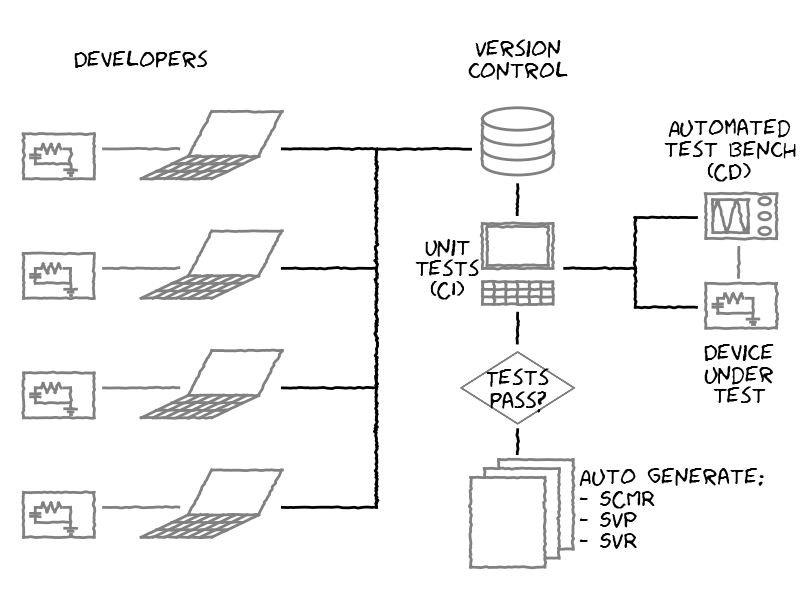
\includegraphics[width=90mm]{agile_setup.png}
	\caption{Agile infrastructure}
\end{figure}

These automated generated outputs still has to comply with the DO-178 requirements on outputs as stipulated in the Annex A of the specification.

To limit the scope of the case study (since it was after all only a student project), only the following deliverables were required:
\begin{itemize}
	\item Plan for software aspects of certification (PSAC)
	\item Software development plan (SDP)
	\item Software requirements data (SRD)
	\item Design description (DD)
	\item Source code
	\item Object code
	\item Software Verification Results (SVR)
	\item Software Accomplishment Summary (SAS)
\end{itemize}

\section{Research design and methodology}

In order to test the effect that a more agile project management approach would have on a project requiring DO-178 certification, a case study was launched. In this case study two 3'rd year student teams developed and delivered a project according to exactly the same specification, with the one team running the agile workflow and the other a more traditional waterfall workflow.  

\begin{figure}[t!]
	\centering 
	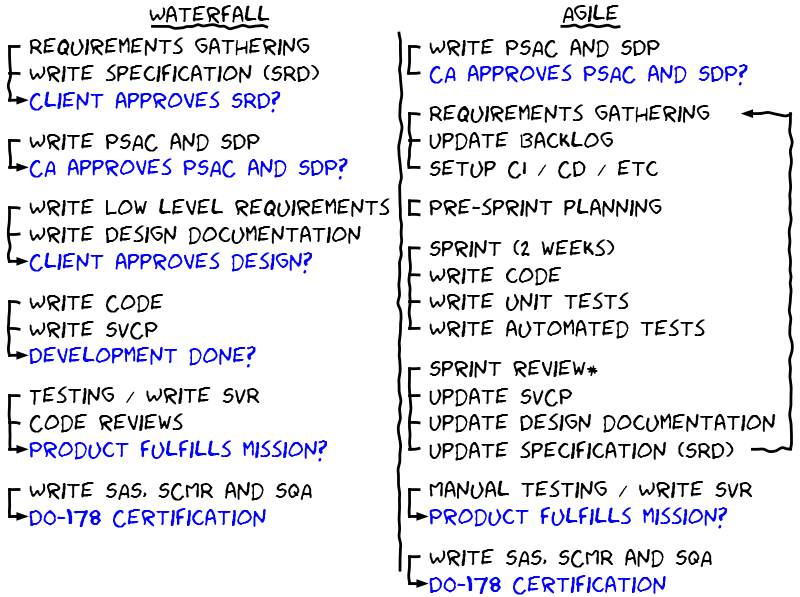
\includegraphics[width=90mm]{agileWaterfallTeamActivities.png}
	\caption{Waterfall vs Agile comparison}
\end{figure}

The teams were tasked with developing group chat functionality for the Linphone open source project \cite{Linphone_2015}, and the final deliverable were measured for robustness of the solution, functionality delivered, maintainability, code bulk and the documentation bulk delivered.

Robustment were determined with independent functional testing of the solution, as well as the amount of unit tests and functional tests each team generated during development. 

Functionality delivered was a simple count against the original specification provided to each team.

Maintainability was determined by calculating the cyclomatic complexity of their code, as well as asking each team to give an estimate as to the effort required to develop additional functionality.

Code bulk is simply the count of lines of code delivered, documentation bulk is the word count of the documentation. Documentation also includes code comments.

Because the teams are not identical, in their size or their capability, a normalization task was given to each team. In this task, they were given exactly the same programming assignment to be completed in roughly half a day. The teams were measured on how long they took to complete the task and the quality of their final solution (how many bugs were still present). All case study metrics were then scaled against the results of this normalization exercise.

\section{Case study}

The 3rd year computer science students at the University of Pretoria has a year long subject where they complete a project as a team. This is the students first substantial project working as a team. These students are presented with a list of projects they are allowed to tender for, on this list was included two projects for this case study. Both projects listed exactly the same requirements, but it was stipulated that the one project will be run agile and the other waterfall. So some self selection of the students biased towards agile or waterfall workflows are present in the case study. For the tenders, six teams applied, three for each project. The two best applications were selected for this case study.

The teams were guided by faculty towards the completion of their projects (Dr Solms, Stacy and Freda), and monitored for their ability to work together. The waterfall team presented better in this regards with a more dilligent work ethic, and better team cohesion. The agile team had difficulties assigning roles to the team members but later in the project managed to pull together.

The agile team selected consists of six members and the waterfall team selected consists of five members. Team members from both teams have some experience with class projects they have completed, served as tutors in various subjects but haven't worked on any large scale projects (multiple team members). Neither teams have experience with DO-178 certified software projects, and have only a theoretical understanding of agile and waterfall development practices.  

The teams submitted their tenders at the beginning of May 2015, and were notified of their successful application a week later. The first meeting between the teams and the client took place end of May after which the teams started their projects in earnest. 


The project  assigned was for the development of features on the linphone open source project (TODO reference). Linphone is a mature Android application (TODO say more about linphone). The teams had about 6 months time from then on to complete the following list of identical requirements:
\\
\begin{itemize}
	\item Group chat (Invite additional members to a chat, all members receive chats)
	\item Secure group chat (AES256)
	\item Creation and deletion of groups
	\item Voice record and send over IM
	\item Rework the messaging user interface
	\begin{itemize}
		\item Improve spacing between words
		\item Make the text bigger
		\item Block indents required to better specify who said what
		\item Presence indication to show a remote user is typing
		\item User picture portraits
	\end{itemize}
\end{itemize}

Emphasis was placed with the student groups that the core requirement was the group chat functionality, then the encryption of the chats, and that all other requirements were of lesser importance. This was done to ensure both groups progress through the work similarly and that one group don't complete the easy work and the other the more difficult work items, which would make comparison difficult.  

%\begin{figure}[t!]
%	\centering 
%	\includegraphics[width=90mm]{progress.png}
%	\caption{Progress of the teams (TODO)}
%\end{figure}

\section{Normalisation of the groups}

The results from the case study were normalised to account for the differing skill levels of the student teams. The normalisation was done by having each team do a sample project taking 4 hours, and comparing their output. The students delivered the executable, source code, a user manual and the code had to be commented sufficiently.

\begin{figure}[t!]
	\centering 
	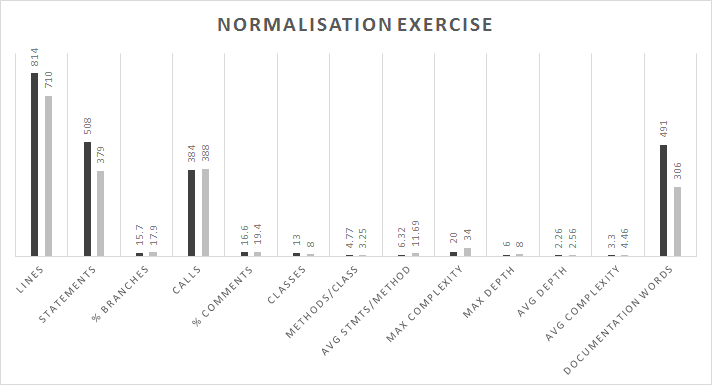
\includegraphics[width=90mm]{NormalisationExercise.png}
	\caption{Normalisation results}
\end{figure}  

From the normalisation exercise we can account for the differences in the teams by a factor of 26\% for code bulk, and 38\% for documentation word count. Qualitative comparison for instance documentation quality and robustness of their solution is difficult to account for but it is assumed the difference will be about the same as it is too a function of the teams ability and work ethic.

\section{Results}

The final projects were demonstrated by the students, and all deliverables and project artifacts were handed in. In the figure we can see a comparison of the projects on the metrics of:
\begin{itemize}
	\item Lines of code
	\item Lines of comments
	\item Cyclomatic complexity
	\item Documentation word count
\end{itemize}

From these quantitative measures the teams differed by approximately 50\%, that is the waterfall team delivered twice as many lines of code, documentation and working functionality than the agile team. From the normalisation exercise to account for the difference in team strengths we would have expected a difference closer to half of that. 

\begin{figure}[t!]
	\centering 
	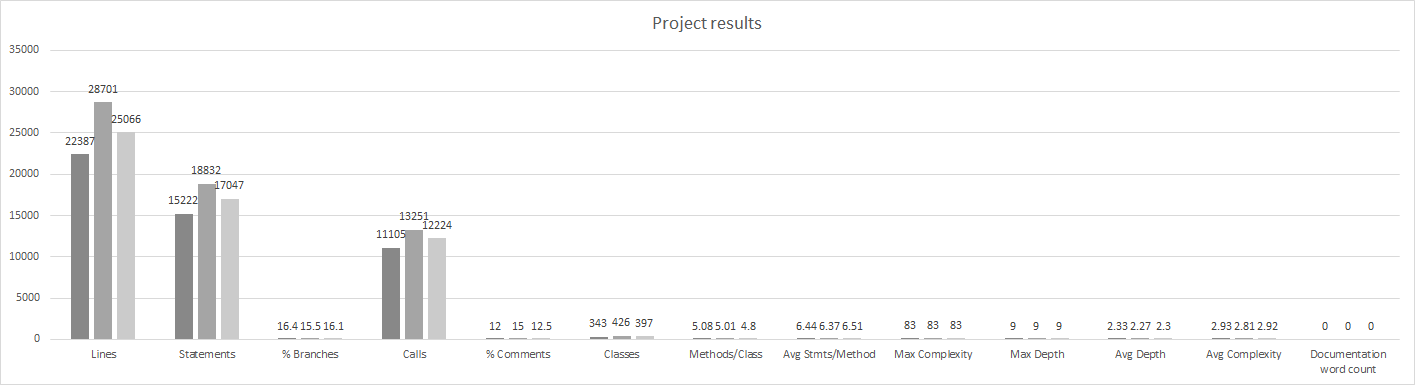
\includegraphics[width=90mm]{Project results.png}
	\caption{Project results}
\end{figure}


With project completion both teams demonstrated their projects to industry and their academic study leaders. During the demonstration the waterfall teams project delivered more functionality and held up better under testing. On the other hand the agile team project had a better user experience compared to the waterfall project. 

\section{Dificulties the teams encountered} 

Both teams struggled with the amount of code already present in linphone, and finding their way in the project (this case study was a brown fiels project). The teams also struggled somewhat with building and running the linphone project. Both teams also struggled a bit with git, especially with linphones use of git submodules which can be a tricky subject.

Furthermore each team struggled with different aspects specific to their project methodology:

\subsection{Waterfall team}
The waterfall team had what is typically known as an integration party, where the work items from each team member is added together at the end. The estimated work effort to get all these elements to work together was underestimated causing some last minute stress on the team.
\\ 
The team also underestimated the amount of time required for sufficient testing at the end with proper acceptance test procedures.

\subsection{Agile team}
The agile team had trouble delivering functioning code with each sprint. This was due perhaps to lack of understanding of agile workflow, poor work ethic or overestimating their ability with each sprint. This was also further caused because of their difficulty with setting up a continuous integration server.
\\
The team had difficulty setting up a continuous integration server, this was mostly due to the complicated build setup the linphone project requires.
\\ 
The team also had difficulty with a test driven development methodology, and subsequently not enough unit and functional tests were written during development.

\section{Conclusion}
One cannot generalise from a single case study, and as such this study cannot speak with sufficient authority on the effectiveness of agile development methodologies versus traditional waterfall methodologies. Nevertheless this study does hint that agile development is not a silver bullet for all project types, and this might explain its poor adoption in highly regulated and safety critical industries. 

There is value in the methodology that waterfall forces on a team, especially in getting a team to do proper scoping of the project and in doing so getting comfortable with the domain of the work.

This case study was uncontrolled for the effect that a green field vs brown field project have on the result. The case study was done on a very mature and large existing project. Furthermore some of the difficulties the teams faced stemmed from their inexperience, which might also affect the results of this study. 

The true value this case study provides is as a reference for further investigation into the effectiveness of agile and waterfall methodologies, and some of the pitfalls one can avoid when conducting such a study. Additional studies can be used to compare results with this one, and in so doing build a case for the effectiveness in either agile or waterfall development practises, especially in safety critical and regulated environments. 



% use section* for acknowledgement
\section*{Acknowledgment}


The authors would like to thank...

\begin{itemize}
	\item Mr Kobus Steyn for his contribution on DO-178 considerations and best practices.
	\item Ms Vreda Pieterse (lecturer) and Ms Stacy Omeleze (assistant lecturer) for their help with running the case study.
\end{itemize}

The following B.Sc Comp Sci students for participating in the study:
\begin{itemize}
	\item Patience Mtsweni
	\item Lerato Molokomme
	\item Tsepo Ntsaba
	\item Mpedi Mello
	\item Lutifyya Razak
	\item Ephiphania Munava
	\item Izak Blom
	\item David Breetzke
	\item Paul Engelke
	\item Prenolan Govender
	\item Jessica Lessev
	\\ 
\end{itemize}
This study was completed as partial fulfilment of the requirements for the degree of: \\
\begin{center}Master of Engineering (MEM)\\
in the\\

GRADUATE SCHOOL OF TECHNOLOGY MANAGEMENT,\\
FACULTY OF ENGINEERING, BUILT ENVIRONMENT AND INFORMATION TECHNOLOGY,\\
UNIVERSITY OF PRETORIA
\end{center}

\bibliographystyle{abbrv}
\bibliography{ref}  

% That's all folks!
\end{document}
